\documentclass{article}
\usepackage{geometry}
\geometry{a4paper, margin=1in}
\usepackage{graphicx}
\usepackage[colorlinks=true, linkcolor=blue, citecolor=blue, urlcolor=blue]{hyperref}
\usepackage{listings}
\usepackage{xcolor}
\usepackage{amsmath}
\usepackage{enumitem}
\usepackage{float}

\lstset{
    language=NASM,
    basicstyle=\ttfamily\footnotesize\selectfont, % use the selected monospaced font
    backgroundcolor=\color{white},
    keywordstyle=\color{blue},
    commentstyle=\color{gray},
    stringstyle=\color{red},
    numbers=left,
    numberstyle=\tiny\color{gray},
    stepnumber=1,
    numbersep=10pt,
    frame=single,
    breaklines=true,
    captionpos=b,
    tabsize=4
}

\title{Assignment 1: v02 - Loading Data from Sector 37}
\author{
    [Welby Seely] \\
    \texttt{[wseely@emich.edu]}
}
\date{\today}

\begin{document}

    \maketitle
    \section{Intro}\label{sec:intro}
    The v1 version of the bootloader was updated to load all data from sector 37.
    Makefile and original assembly file was updated accordingly.

    The program uses VGA graphics mode with 320 x 200 resolution and 256 colors to display a
    custom `W' logo and the required text for the splash screen.

    After entering any key, the program switches to text mode and display a magenta `\$' and a
    blinking cursor.

    This fulfills the basic requirements:

    \begin{itemize}
        \item The build process writes the MBR in sector 0, and the data into sector 37.
        \item When booted, it displays a welcome message.
        \item It waits for a key stoke.
        \item After key stoke, the welcome is cleared.
        \item Then a command prompt `\$' at the top left corner followed by a blinking cursor (not required, but left in).
    \end{itemize}

    \section{Loading from sector 37}\label{sec:reqs}
    int13 function 2 was used to load sector 37.

    Equations:
    \begin{itemize}
        \item Physical Sector: \verb|(L % N) + 1|.
        \item Cylinder: \verb|(L / N) / S|.
        \item Head: \verb|(L / N) % S|.
    \end{itemize}
    Where \verb|L| is the logical sector, \verb|T| is the cylinders (tracks) per side, and \verb|S| is the number of sides.

    \begin{itemize}
        \item Sector: \verb|37 / 18 + 1 = 2|
        \item Cylinder: \verb|37 / 18 / 2 = 1|
        \item Head: \verb|37 / 18 % 2 = 0|
    \end{itemize}

    Based on these parameters, wrote the load\_sector subroutine:
    \begin{lstlisting}
        load_sector:
            mov bx, 0x0000
            mov es, bx
            mov bx, 0x7e00
            mov ah, READ_SECTORS
            mov al, 1
            mov ch, 1 ; cylinder
            mov cl, 2 ; sector
            mov dh, 0 ; head number
            mov dl, 0
            int BIOS_FLOPPY
            ret
    \end{lstlisting}

    \section{Screenshots}\label{sec:screenshots}
    Screenshots of the splash screen and the prompt screen are provided.

    \begin{figure}[H]  % [H] forces the figure to appear here
        \centering
        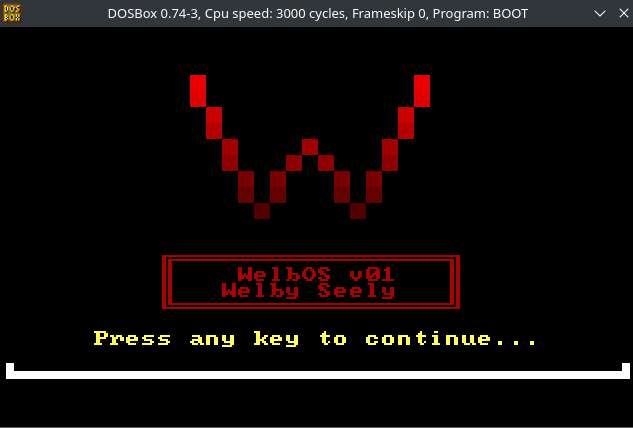
\includegraphics[width=\textwidth]{splash-screen} % Scales image to document width
        \caption{Custom splash screen, complete with logo in graphics mode}
        \label{fig:1}
    \end{figure}

    \begin{figure}[H]  % Ensures figure appears right here
        \centering
        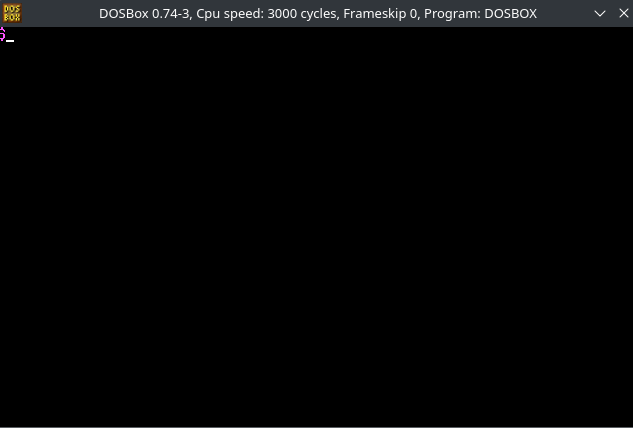
\includegraphics[width=\textwidth]{prompt} % Scales image to document width
        \caption{Prompt with \$ and a blinking cursor}
        \label{fig:2}
    \end{figure}

    \section{Appendix 1: Source Code}\label{sec:appendix_1}
    \begin{lstlisting}[caption={os623V02.asm listing}, captionpos=t]
       bits 16
        BIOS_VIDEO          equ 0x10
        DISPLAY_FUN         equ 0x13

        FUN_VIDEO_MODE      equ 0x0000
        VGA_MODE            equ 0x0013

        BIOS_FLOPPY         equ 0x0013
        READ_SECTORS        equ 0x0002

        VGA_DISPLAY_WIDTH   equ 320
        DISPLAY_WIDTH       equ 80
        DISPLAY_HEIGHT      equ 25
        VGA_TXT_DISP_WIDTH  equ 40
        VGA_TXT_DISP_HEIGHT equ 25
        MESSAGE_ROW         equ VGA_TXT_DISP_HEIGHT / 2 + 3
        LINE_ROW_TOP        equ MESSAGE_ROW - 1
        LINE_ROW_NAME       equ MESSAGE_ROW + 1
        LINE_ROW_BOTTOM     equ LINE_ROW_NAME + 1
        LINE_ROW_ANYKEY     equ LINE_ROW_BOTTOM + 2
        TEXT_MODE           equ 0x03
        MAGENTA_BLACK       equ 0x0D
        WHITE_BLACK         equ 0x0F
        RED_BLACK           equ 0x04
        YELLOW_BLACK        equ 0x0E
        LIGHT_RED           equ 0x0C
        LOGO_START_X        equ (VGA_DISPLAY_WIDTH - (16 * SCALING_FACTOR)) / 2
        LOGO_START_Y        equ (200 - (9 * SCALING_FACTOR)) / 2 -40

        SCALING_FACTOR      equ 0x8
        FALSE               equ 0x00

        BOX_LENGTH          equ 19
        ANYKEY_LENGTH       equ 28
        BITMAP_LENGTH       equ 18
        SHADE_COUNT         equ 9

        ;data refs
        topline             equ 0x7e00
        bottomline          equ topline + 3
        blockline           equ bottomline + 3
        welbos              equ blockline + 3
        name                equ welbos + BOX_LENGTH
        anykey              equ name + BOX_LENGTH
        prompt_sym          equ anykey + ANYKEY_LENGTH
        w_bitmap            equ prompt_sym + 1
        red_shades          equ w_bitmap + BITMAP_LENGTH
        row_colors          equ red_shades + SHADE_COUNT


        %define CENTER_TXT(len) ((DISPLAY_WIDTH - len) / 2)
        %define CENTER_VGA_TXT(len) ((VGA_TXT_DISP_WIDTH - len) / 2)

        org 0x7c00
        jmp short start
        nop

        bsOEM       db "WelbOS v01"         ; OEM String

        start:
            call load_sector

            mov ax, FUN_VIDEO_MODE + VGA_MODE
            int BIOS_VIDEO

            call set_red_gradient_palette
            ;    mov di, LOGO_START_Y * VGA_DISPLAY_WIDTH + LOGO_START_X
            push LOGO_START_X
            push LOGO_START_Y
            call draw_logo

            push RED_BLACK
            push BOX_LENGTH
            push welbos
            push MESSAGE_ROW
            push CENTER_VGA_TXT(BOX_LENGTH)
            call print

            push RED_BLACK
            push BOX_LENGTH - 1               ; Repeat count
            push CENTER_VGA_TXT(BOX_LENGTH)   ; Column
            push LINE_ROW_TOP                ; Row
            push topline                     ; Address of 3-tuple
            call draw_line

            push RED_BLACK
            push BOX_LENGTH
            push name
            push LINE_ROW_NAME
            push CENTER_VGA_TXT(BOX_LENGTH)
            call print

            push RED_BLACK
            push BOX_LENGTH - 1       ; Repeat count
            push CENTER_VGA_TXT(BOX_LENGTH)   ; Column
            push LINE_ROW_BOTTOM     ; Row
            push bottomline             ; Address of 3-tuple
            call draw_line

            push YELLOW_BLACK
            push ANYKEY_LENGTH
            push anykey
            push LINE_ROW_ANYKEY
            push CENTER_VGA_TXT(ANYKEY_LENGTH)
            call print

            push WHITE_BLACK
            push VGA_TXT_DISP_WIDTH - 1       ; Repeat count
            push 0   ; Column
            push LINE_ROW_ANYKEY + 2          ; Row
            push blockline                    ; Address of 3-tuple
            call draw_line

            ; Wait for key press
            mov ah, 0x00
            int 0x16

            ; Switch back to text mode (80x25)
            mov ax, 0x0003
            int BIOS_VIDEO

            call clear_screen

            call set_cursor_pos

            push MAGENTA_BLACK
            push 1
            push prompt_sym
            push 0
            push 0
            call print
        end:
            int 20h

        draw_logo:
            push bp
            mov bp, sp

            mov ax, [bp + 4]
            mov cx, VGA_DISPLAY_WIDTH
            mul cx
            add ax, [bp + 6]
            mov di, ax

            mov ax, 0xA000     ; memory mapped I/O segment for VGA
            mov es, ax

            mov di, LOGO_START_Y * VGA_DISPLAY_WIDTH + LOGO_START_X
            mov si, w_bitmap   ; source bitmap start address

            mov dx, 9                  ; logical row that we're calculating
            push SCALING_FACTOR
        draw_rows:
            mov bx, 9
            sub bx, dx                 ; determine color for this row
            mov bl, [row_colors + bx]  ; store row color in BL (or AL, but we’ll need AL soon)
            mov ax, [si]               ; retrieve pixels for this row

            ; Process 16 pixels
            mov cx, 16
        draw_row:
            shl ax, 1          ; Shift left (test MSB of AX)
            jnc skip_column

            push cx
            push ax
            mov cx, SCALING_FACTOR
            mov al, bl
            rep stosb
            pop ax
            pop cx
            jmp next_column
        skip_column:
            add di, SCALING_FACTOR
        next_column:
            loop draw_row

        scale_vertically:
            add di, 320 - 16 * SCALING_FACTOR ; Move to next VGA row
            pop cx
            dec cx
            cmp cx, 0
            jz next_source_row
            push cx
            jmp draw_rows
        next_source_row:
            add si, 2
            dec dx
            jz logo_done
            push SCALING_FACTOR
            jmp draw_rows
        logo_done:
            pop bp
            ret 4

        draw_line:
            push bp
            mov bp, sp

            ;left edge
            push word [bp + 12]
            push 1
            mov si, [bp + 4]
            push si
            mov si, [bp + 6]
            push si
            mov si, [bp + 8]
            push si
            call print

            ; set up middle loop
            mov ax, 1                           ; break when == to cx
        draw_line_middle:
            mov cx, [bp + 10]
            cmp ax, cx
            je draw_line_right
            push ax

            push word [bp + 12]
            push 1
            mov si, [bp + 4]
            inc si
            push si
            mov si, [bp + 6]
            push si
            mov si, [bp + 8]
            add si, ax
            push si
            call print

            pop ax
            inc ax
            jmp draw_line_middle

        draw_line_right:
            push word [bp + 12]
            push 1
            mov si, [bp + 4]
            add si, 2
            push si
            mov si, [bp + 6]
            push si
            add ax, [bp + 8]                    ; rightmostposition
            push ax
            call print

            pop bp
            ret 10


        set_cursor_pos:
            mov ah, 0x02        ; BIOS function: set cursor position
            mov bh, 0x00        ; Page number (0)
            mov dh, 0x00        ; Row (0)
            mov dl, 0x01        ; Column (1)
            int BIOS_VIDEO
            ret

        set_red_gradient_palette:
            mov dx, 0x3C8   ; VGA color index port
            mov al, 32      ; Start setting colors from index 32
            out dx, al
            inc dx          ; Now dx = 0x3C9 (RGB color data port)

            mov cx, 9       ; 9 shades for 9 rows
            mov si, red_shades
        next_color:
            mov al, [si]    ; Load Red intensity
            out dx, al      ; Set Red value
            xor al, al      ; Set Green=0
            out dx, al
            out dx, al      ; Set Blue=0
            inc si
            loop next_color
            ret

        ; -----------------------------------------------------------------------------
        ; Function: clear_screen
        ; Description: Clears and resets the screen.
        ; Inputs: None.
        ; Outputs: None.
        ; Modifies:
        ;   - AX, BX, CX, DX
        ; Calls:
        ;   - BIOS interrupt 0x10, function 0x06.
        ; -----------------------------------------------------------------------------
        clear_screen:
            mov ah, 0x06            ; BIOS scroll (function 06h)
            mov al, 0               ; Scroll all lines
            mov bh, WHITE_BLACK         ; Attribute
            mov ch, 0               ; Upper-left row
            mov cl, 0               ; Upper-left column
            mov dh, 24              ; Lower-right row
            mov dl, 79              ; Lower-right column
            int BIOS_VIDEO          ; BIOS video interrupt
            ret

        ; -----------------------------------------------------------------------------
        ; Function: load_sector
        ; Description: Loads sector 37 into memory. TODO parameterize
        ; Inputs: None.
        ; Outputs: None.
        ; Modifies:
        ;   - AX, BX, CX, DX, EX
        ; Calls:
        ;   - BIOS interrupt 0x13, function 0x02.
        ; -----------------------------------------------------------------------------
        load_sector:
            mov bx, 0x0000
            mov es, bx
            mov bx, 0x7e00
            mov ah, READ_SECTORS
            mov al, 1
            mov ch, 1
            mov cl, 2
            mov dh, 0
            mov dl, 0
            int BIOS_FLOPPY
            ret

        ; -----------------------------------------------------------------------------
        ; Function: print
        ; Description: Prints a string to the console.
        ; Inputs:
        ;   - [sp+4] Column position to begin writing the string.
        ;   - [sp+6] Row position to begin writing the string.
        ;   - [sp+8] Memory address location of the string.
        ;   - [sp+10] Length of the string.
        ; Outputs: None.
        ; Modifies:
        ;   - AX, BX, CX, DX
        ; Calls:
        ;   - BIOS interrupt 0x10, function 0x13.
        ; -----------------------------------------------------------------------------
        print:
            push bp ; save bp for the return
            mov  bp, sp ; update bp to create a new "stack frame"

            mov bl, [bp+12]        ; Attribute (lightgreen on black)
            mov cx, [bp+10]        ; length of the string
            mov si, [bp+8]         ; address of the string
            mov dh, [bp+6]         ; row position
            mov dl, [bp+4]         ; column position

            ; We need ES:BP provides the pointer to the string - load the data segment (DS) base into ES
            push ds
            pop es

            mov  ah, DISPLAY_FUN    ; BIOS display string (function 13h)
            mov  al, 0              ; Write mode = 1 (cursor stays after last char
            mov  bh, 0              ; Video page
            mov  bp, si             ; Put offset in BP (ES:BP points to the string)
            int  BIOS_VIDEO

            pop bp                 ; Restore stack frame
            ret 10

        ; Pad to 512 bytes for an MBR:
        padding times 510 - ($ - $$) db 0

        ; Optional boot signature:
        bootSig db 0x55, 0xAA

    \end{lstlisting}

    \begin{lstlisting}[caption={loaderV02.asm listing}, captionpos=t]
        bits 16

        org 0x7e00
        topline             db 0xC9
                            db 0xCD
                            db 0xBB
        bottomline          db 0xC8
                            db 0xCD
                            db 0xBC
        blockline           db 0xDE
                            db 0xDC
                            db 0xDD
        welbos              db 0xBA, `    WelbOS v01   `, 0xBA
        name                db 0xBA, `   Welby Seely   `, 0xBA
        anykey              db "Press any key to continue..."
        prompt_sym          db '$'
        w_bitmap db 02h, 80h
                 db 02h, 80h
                 db 04h, 40h
                 db 04h, 40h
                 db 08h, 21h
                 db 88h, 22h
                 db 50h, 14h
                 db 50h, 14h
                 db 20h, 08h
        red_shades db 58, 55, 50, 45, 40, 35, 30, 25, 20; Bright to dark red
        ; Row color table, from top to bottom row
        row_colors db 32, 33, 34, 35, 36, 37, 38, 39, 40  ; Use only custom red shades
    \end{lstlisting}

    \begin{lstlisting}[caption={Makefile listing}, captionpos=t]
        VER			= V02
        ASM			= nasm
        ASMFLAGS	= -f bin
        IMG			= a.img

        MBR			=  os623V.asm
        MBR_SRC		= $(subst V,$(VER),$(MBR))
        MBR_BIN		= $(subst .asm,.bin,$(MBR_SRC))

        DATA_SRC	=  loaderV02.asm
        DATA_BIN	=  data.bin


        .PHONY : everything

        .PHONY : all everything clean reset blankimg

        all: everything

        everything : $(MBR_BIN) $(DATA_BIN)
         ifneq ($(wildcard $(IMG)), )
         else
                dd if=/dev/zero of=$(IMG) bs=512 count=2880
         endif

                dd if=$(MBR_BIN) of=$(IMG) bs=512 count=1 conv=notrunc
                dd if=$(DATA_BIN) of=$(IMG) bs=512 seek=37 conv=notrunc

        $(MBR_BIN) : $(MBR_SRC)
        #	nasm -f bin $< -o $@
            $(ASM) $(ASMFLAGS) $< -o $@

        $(DATA_BIN) : $(DATA_SRC)
            $(ASM) $(ASMFLAGS) $< -o $@

        clean :
            rm -f $(MBR_BIN) $(DATA_BIN)

        reset:
            rm -f $(MBR_BIN) $(DATA_BIN) $(IMG)

        blankimg:
            dd if=/dev/zero of=$(IMG) bs=512 count=2880
    \end{lstlisting}

\end{document}
